\section{Durchführung und Auswertung}

\subsection{Charakterisierung des Pumplasers}


\subsubsection{Aufbau und Durchführung}

\subsubsection{Auswertung}

\begin{figure}[H]
\begin{center}
  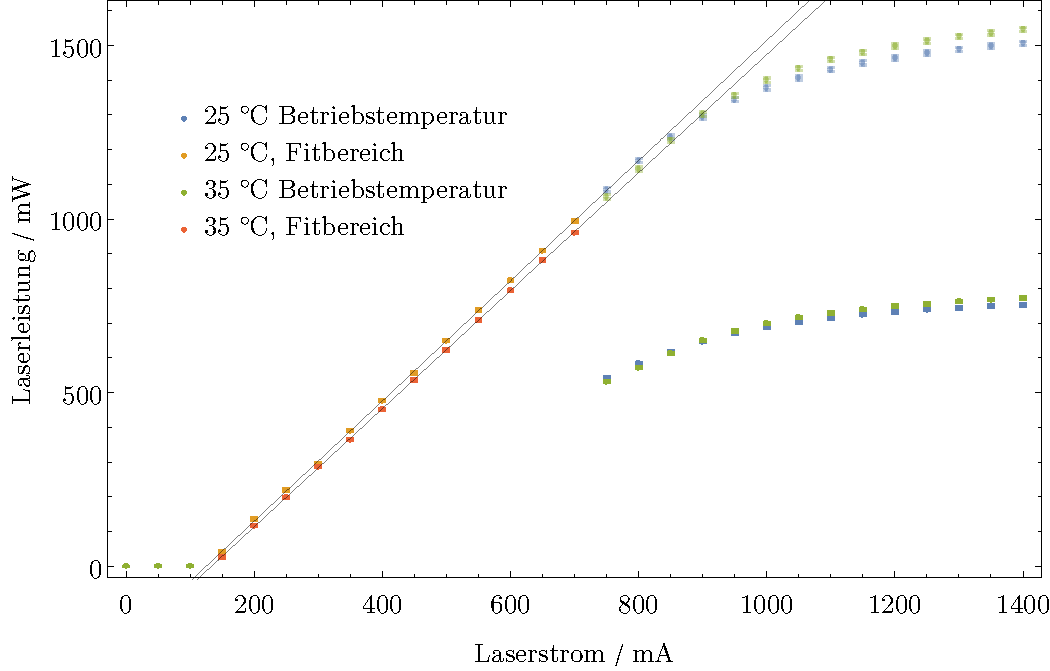
\includegraphics[width=\textwidth]{PI_blau.pdf}
  \caption{PI-Kennlinie des blauen Pumplasers bei 25\grad und 35\grad
  Betriebstemperatur. Der modulationsfreie Bereich wurde mit $y=a(x-b)$
  gefittet, um die Laserschwelle~$b$ und die Effizienz~$a$ zu bestimmen. Im
  Bereich der Modulation mit einer Pulsweite von 50\,\% über 700\,mA Laserstrom ist durch eine
  Multiplikation mit Faktor 2 angedeutet, bei welcher Leistung der Laser
  transient betrieben wird.}
  \label{img:PI_blau}
\end{center}

\end{figure}

Abbildung \ref{img:PI_blau} zeigt die beiden Kennlinien, die bei 25\grad und 35\grad Lasertemperatur
aufgenommen wurde.
Der Fehler der Laserleistung wurde aus der minimalen und maximalen Leistung abgeschätzt, die für die
einzelnen Messpunkte gemessen wurde.
Diese Schwankungen wurden mit höherem Betriebsstrom stärker.
Der Fehler auf den Laserstrom wird als vernachlässigbar klein angenommen.

 Nur der modulationsfreie Bereich von der Laserschwelle bis 700\,mA Laserstrom
zeigt einen linearen Verlauf.
Deshalb wurde der lineare Fit auf diesen Bereich beschränkt.
Da die Modulation des Lasers mit einer Pulsweite von 50\,\% stattfindet, hätte mit einer
Verdoppelung der Leistungen im Bereich über 700\,mA eine Erweiterung des Fitbereichs bis ca. 850\,mA
durchgeführt werden können. Erst bei Betriebsströmen über 850\,mA geht die Leistung deutlich in
Sättigung.

Tabelle \ref{tab:Fits_PI_blau} zeigt die Ergebnisse der beiden Fits.


\begin{table}[htb]
\caption{Ergebnisse der Fits der PI-Kennlinien des Pumplasers mit $y=a(x-b)$.}
\begin{center}
\begin{tabular}{|c|c|}
\hline
\textbf{25\grad} &  \\ \hline
$a$ & 1.730\,$\pm$\,0.005\,mW\,/\,mA \\ \hline
$b$ & 124.7\,$\pm$\,1.0\,mA \\ \hline
\textchi$^2$ & 16.0142 \\ \hline
\textchi$^2$/\,DoF & 1.60142 \\ \hline
 &  \\ \hline
\textbf{35\grad} &  \\ \hline
$a$ & 1.699\,$\pm$\,0.005\,mW\,/\,mA \\ \hline
$b$ & 133.0\,$\pm$\,1.0\,mA \\ \hline
\textchi$^2$ & 7.24023 \\ \hline
\textchi$^2$/\,DoF & 0.724023 \\ \hline
\end{tabular}
\end{center}
\label{tab:Fits_PI_blau}
\end{table}

\FloatBarrier
 